\section{The \commonalities Approach}
\label{chap:improvement:commonalities}

\mnote{Approach overview}
We have motivated the idea of representing common concepts of different metamodels in terms of \commonalities in explicit \conceptmetamodels rather than implicitly encoding them in direct consistency relations between the \concretemetamodels.
In the following, we discuss the specification of \conceptmetamodels and the notion of manifestation relations in more detail.
We also depict how further benefits can be generated by composing \conceptmetamodels in terms of defining a hierarchy of them.
We call this approach of defining and composing \conceptmetamodels of \commonalities the \emph{\commonalities approach}.
The mitigation of trade-offs between quality properties as the central benefit of the approach is given by the inherent possibility to achieve a specific kind of tree topology, which we derive from the approach before discussing different options for its operationalization.


\subsection{Concept Metamodels}

\mnote{Structure of metamodels}
The inherent benefits of the \commonalities approach are given by the definition of additional \conceptmetamodels, across which consistency relations are expressed instead of defining consistency relations between the \concretemetamodels.
Conceptually, it is not that relevant how the structure of these \conceptmetamodels and of the manifestation relations to the \concretemetamodels actually is.
Still, we discuss how elements can be represented as \commonalities in a \conceptmetamodel and which relations beyond pure redundancies representing exactly the same information they may express.

\begin{figure}
    \centering
    \newcommand{\vdistance}{12em}
\newcommand{\hdistance}{23em}
\newcommand{\innerhdistance}{7.6em}
\newcommand{\classwidth}{4.7em}
\newcommand{\labeldistance}{0.9em}
\newcommand{\mmborder}{0.9em}
\newcommand{\referenceshift}{0.9em}

\begin{tikzpicture}

\pgfdeclarelayer{bg}
\pgfsetlayers{bg,main}


% METACLASSES

\umlclassvarwidth{java_class}{}{Class}{
name\\
packageName
}{\classwidth}  

\umlclassvarwidth[, right=\innerhdistance of java_class.north, anchor=north]{java_field}{}{Field}{
name\\
}{\classwidth} 

\umlassociationfromto{([yshift=\referenceshift]java_field.west-|java_class.east) -- node[uml cardinality start, pos=0, above right] {$1$} node[uml cardinality end, pos=1, above left] {$*$} ([yshift=\referenceshift]java_field.west)}
\umlassociationfromto{([yshift=-\referenceshift]java_field.west) -- node[uml cardinality start, pos=0, above left] {$*$} node[uml role end, pos=1, below right] {type} node[uml cardinality end, pos=1, above right] {$1$} ([yshift=-\referenceshift]java_field.west-|java_class.east)}

\umlclassvarwidth[, below right=5em and \hdistance of java_class.north, anchor=north]{uml_class}{}{Class}{
name\\
}{\classwidth} 

\umlclassvarwidth[, left=\innerhdistance of uml_class.north, anchor=north]{uml_association}{}{Association}{
name\\
}{\classwidth}

\umlclassvarwidth[, above=5em of uml_class.north, anchor=north]{uml_package}{}{Package}{
name\\
}{\classwidth}

\umlassociationfromto{([yshift=\referenceshift]uml_association.east) -- node[uml cardinality start, pos=0, above right] {$*$} node[uml role end, pos=1, below left] {from} node[uml cardinality end, pos=1, above left] {$1$} ([yshift=\referenceshift]uml_class.west)}
\umlassociationfromto{([yshift=-\referenceshift]uml_association.east) -- node[uml cardinality start, pos=0, above right] {$*$} node[uml role end, pos=1, below left] {to} node[uml cardinality end, pos=1, above left] {$1$} ([yshift=-\referenceshift]uml_class.west)}
\umlassociationfromto{(uml_package.south) -- node[uml cardinality start, pos=0, below left] {$1$} node[uml role end, pos=1, above right] {classes} node[uml cardinality end, pos=1, above left] {$*$} (uml_class.north)}

\umlclassvarwidth[, above right=\vdistance and 0.5*\hdistance-0.5*\innerhdistance of java_class.north, anchor=north]{oo_class}{}{Class\vphantom{p}}{
name\\
}{\classwidth} 

\umlclassvarwidth[, below=5em of oo_class.north, anchor=north]{oo_association}{}{Association}{
name\\
}{\classwidth}

\umlclassvarwidth[, right=1.2*\innerhdistance of oo_class.north, anchor=north]{oo_package}{}{Package}{
name\\
}{\classwidth}

\umlassociationfromto{([xshift=-0.8*\referenceshift]oo_class.south) -- node[uml cardinality start, pos=0, below right] {$1$} node[uml role end, pos=0, below left] {from} node[uml cardinality end, pos=0, above right] {$*$} ([xshift=-0.8*\referenceshift]oo_association.north)}
\umlassociationfromto{([xshift=1.2*\referenceshift]oo_association.north) -- node[uml cardinality start, pos=0, above left] {$*$} node[uml role end, pos=1, below right] {to} node[uml cardinality end, pos=1, below left] {$1$} ([xshift=1.2*\referenceshift]oo_class.south)}
\umlassociationfromto{(oo_package.west) -- node[uml cardinality start, pos=0, below left] {$1$} node[uml role end, pos=1, above right] {classes} node[uml cardinality end, pos=1, below right] {$*$} (oo_class.east)}


% METAMODELS

\coordinate (java_label_coordinate) at ([yshift=\labeldistance]java_class.north west);
\node[mmlabel, anchor=west] (java_label) at (java_label_coordinate) {Java};

\coordinate (uml_label_coordinate) at ([yshift=\labeldistance]uml_package.north east);
\node[mmlabel, anchor=east] (java_label) at (uml_label_coordinate) {UML};

\coordinate (oo_label_coordinate) at ([yshift=\labeldistance]$(oo_class.north)!0.5!(oo_package.north)$);
\node[mmlabel, anchor=center] (oo_label) at (oo_label_coordinate) {Object-oriented Design};

\begin{pgfonlayer}{bg}
    \node[mmbg, fit=(java_class)(java_field)(java_label_coordinate), inner sep=\mmborder] (java) {};
    \node[mmbg, fit=(uml_class)(uml_package)(uml_association)(uml_label_coordinate), inner sep=\mmborder] (uml) {};
    \node[conceptmmbg, minimum width=11.5em, fit=(oo_class)(oo_association)(oo_package)(oo_label_coordinate), inner sep=\mmborder] (oo) {};
\end{pgfonlayer}


% CONSISTENCY RELATIONS

\draw[manifests relation] ([xshift=-0.48*\classwidth]oo_class.south) -- node[manifests relation, above, sloped] {\manifestslabel} (java_class);
\draw[manifests relation] ([xshift=0.48*\classwidth]oo_class.south) -- node[manifests relation, above, sloped] {\manifestslabel} (uml_class);
\draw[manifests relation] (oo_association) -- node[manifests relation, above, sloped] {\manifestslabel} (java_field);
\draw[manifests relation] (oo_association) -- node[manifests relation, above, sloped] {\manifestslabel} (uml_association);
\draw[manifests relation] (oo_package) -- node[manifests relation, above, sloped] {\manifestslabel} (uml_package);

\end{tikzpicture}

    \caption[Multiple \commonality example for object-oriented design]{\Conceptmetamodel for object-oriented design with a \texttt{Class}, an \texttt{Association} and a \texttt{Package} \commonality and its relations to the \concretemetamodels \gls{UML} and Java with a different representation of associations as fields and packages as attributes of classes in Java.}
    \label{fig:improvement:multiple_commonalities_example}
\end{figure}

\mnote{Representation of packages}
\autoref{fig:improvement:multiple_commonalities_example} depicts an extension of the example given in \autoref{fig:improvement:one_commonality_example}.
In addition to classes, it contains the representation of packages and associations.
A package is represented as a dedicated \metaclass in the \gls{UML}, which references the classes contained in that package.
Java, however, does not have an explicit representation of packages but encodes them into the package names specified within classes and, additionally, represents them in a folder structure in which the source code files of the classes are persisted.
A \conceptmetamodel used to preserve consistency between packages represented in the \gls{UML} and Java must represent this information in any way such that changes in Java code can be propagated into a \gls{UML} model to preserve their consistency and vice versa.
To sketch an extreme, this could even be achieved with some string attribute in the \conceptmetamodel that encodes this information in such a unique way that the necessary information for both instances of the \concretemetamodels can be generated.
Actually, a \conceptmetamodel should represent such information in a reasonable structure, whose concrete characteristics have to be defined by the transformation developer.
For packages, either the representation of Java as attributes of classes or the representation of the \gls{UML} as a dedicated \metaclass can be chosen.
In the given example, we define packages in the \conceptmetamodel as explicit \metaclasses, as this makes the containment structure of classes in packages explicit.
In addition, in the complete \gls{UML} and Java metamodels packages are represented hierarchically, which is also easier to express as a relation between dedicated elements rather than their implicit encoding in the package names of classes.

\mnote{Representation of associations}
Associations in the \gls{UML} are used to define relations between classes.
Each association references two classes, denoting from which class to which class the association is defined.
Java does not provide an explicit representation of associations, which usually results in their implicit representation as fields of the class from which the association is defined and having the type of the class to which it is defined.
In the example, we have chosen to represent an association in the \conceptmetamodel explicitly.
Fields can be related to further elements than associations in the complete Java and \gls{UML} metamodels.
Thus, having this distinction within the \conceptmetamodel gives it more semantics.
In addition, we have chosen that the class from which the association is defined references the association instead of having this reference in the opposite direction as in the \gls{UML} metamodel.
No matter whether this is beneficial or not, all information that is necessary to keep Java fields and \gls{UML} associations consistent is represented by the \conceptmetamodel.
It shows that for a \conceptmetamodel even a representation that differs from all its manifestations can be chosen.

\mnote{General rule for \conceptmetamodels}
As mentioned before, the only requirement to a \conceptmetamodel is that it must be able to represent all information that is necessary for defining manifestation relations to the \concretemetamodels, such that they are able to preserve consistency according to some consistency relation between the \concretemetamodels.
A general but rather informal rule, which has shown to be beneficial in the implementation of a case study for our evaluation, is to select the semantically richest among different representation options.
In the example, we have thus chosen to represent packages explicitly instead of implicitly encoding them in package names of classes.
This improves expressiveness of the \conceptmetamodel and makes its information easier to use for defining manifestation relations without interpreting implicitly encoded information in each of these relations.

\mnote{Reuse of existing metamodels}
Instead of defining a new \conceptmetamodel, it is, of course, also possible to use an existing metamodels as a \conceptmetamodel.
For example, the \gls{UML} may be considered a suitable \conceptmetamodel for object-oriented design.
Doing so does not conflict in any way with the goals of the \commonalities approach.
Such a metamodel can then either only be considered a \conceptmetamodel whose instances are, by accident, also used by developers, or it can be considered both a \conceptmetamodel and a \concretemetamodel with a one-to-one manifestation relation between them.
This is only a conceptual differentiation with no practical impact.
Only for the approach operationalization, which we discuss later, it has to be considered whether instances of a \conceptmetamodel may actually be relevant during productive use or not.


\subsection{Composition of Concepts}
\label{chap:improvement:commonalities:composition}

\mnote{Multiple \commonalities}
We have so far discussed the idea of defining an additional \conceptmetamodel to represent the common concepts of two or more \concretemetamodels.
For the depicted example for Java and the \gls{UML}, it seems reasonable to group the common concepts in object-oriented design in such a metamodel.
In \autoref{fig:improvement:running_example}, we have also considered \gls{PCM} components and their consistency relations to classes in the \gls{UML} and Java.
Although we could define a component \commonality for \gls{PCM} components and classes in the \gls{UML} and Java and consider this \commonality next to the class \commonality for \gls{UML} and Java classes, we will likely not do so because of several drawbacks.
First, a component \commonality does, semantically, not fit into the discussed \conceptmetamodel for object-oriented design. Thus, the \conceptmetamodel would have to be considered broader, potentially as one generic \conceptmetamodel.
Second, and more importantly, such a construction would introduce further redundancies, as the relation between classes in the \gls{UML} and Java would be expressed via the two \commonalities for classes and components.

\mnote{Monolithic \commonalities}
To solve the problem of a redundant specification of the relation between classes in the \gls{UML} and Java via a class and a component \commonality, we could combine these two \commonalities to a single one, representing all necessary common information.
If, however, further elements share information with classes and components, they also have to be merged into the same \commonality.
In the extreme case, this could result in only having one large \commonality that is able to represent all related information.
The manifestation relations would then have to make all kinds of distinctions based on the information given in such a monolithic \commonality.

\mnote{Exemplary \commonality hierarchy}
An intuitive solution for the example scenario is to not consider classes in the \gls{UML} and Java as manifestations of a component \commonality but to consider the class \commonality as a manifestation of the component \commonality.
Then the relation between classes in the \gls{UML} and Java is still represented across one specific class \commonality, whereas the manifestation relation of the component \commonality only has to be defined for the concept of classes instead of their concrete manifestations.

\begin{figure}
    \centering
    \newcommand{\vdistance}{7em}
\newcommand{\hdistance}{13em}
\newcommand{\classwidth}{5.5em}
\newcommand{\labeldistance}{1em}
\newcommand{\labelshift}{0.3*\classwidth}
\newcommand{\mmborder}{1em}

\begin{tikzpicture}

\pgfdeclarelayer{bg}
\pgfsetlayers{bg,main}


% METACLASSES

\umlclassvarwidth{java_class}{}{Class}{
name\\
}{\classwidth}  

\umlclassvarwidth[, right=0.8*\hdistance of java_class.north, anchor=north]{uml_class}{}{Class}{
name\\
}{\classwidth} 

\umlclassvarwidth[, above right=\vdistance and 0.5*\hdistance of java_class.north, anchor=north]{oo_class}{}{Class\vphantom{p}}{
name\\
}{\classwidth} 

\umlclassvarwidth[, right=\hdistance of oo_class.north, anchor=north]{pcm_component}{}{Component}{
name\\
}{\classwidth} 

\umlclassvarwidth[, above right=\vdistance and 0.5*\hdistance of oo_class.north, anchor=north]{component_component}{}{Component}{
name\\
}{\classwidth}

% METAMODELS

\coordinate (java_label_coordinate) at ([yshift=\labeldistance]java_class.north west);
\node[mmlabel, anchor=west] (java_label) at (java_label_coordinate) {Java};

\coordinate (uml_label_coordinate) at ([yshift=\labeldistance]uml_class.north east);
\node[mmlabel, anchor=east] (uml_label) at (uml_label_coordinate) {\acrshort{UML}};

\coordinate (oo_label_coordinate) at ([xshift=-4*\labelshift,yshift=\labeldistance]oo_class.north);
\node[mmlabel, anchor=west, align=left] (oo_label) at ([xshift=-0.5em, yshift=-0.7em]oo_label_coordinate) {Object-oriented\\ Design};

\coordinate (pcm_label_coordinate) at ([yshift=\labeldistance]pcm_component.north east);
\node[mmlabel, anchor=east] (pcm_label) at (pcm_label_coordinate) {\acrshort{PCM}};

\coordinate (component_label_coordinate) at ([yshift=\labeldistance]component_component.north);
\node[mmlabel, anchor=center] (component_label) at (component_label_coordinate) {Component-based Design};

\begin{pgfonlayer}{bg}
    \node[mmbg, fit=(java_class)(java_label.west), inner sep=\mmborder] (java) {};
    \node[mmbg, fit=(uml_class)(uml_label.east), inner sep=\mmborder] (uml) {};
    \node[conceptmmbg, fit=(oo_class)(oo_label_coordinate), inner sep=\mmborder] (oo) {};
    \node[mmbg, fit=(pcm_component)(pcm_label.east), inner sep=\mmborder] (pcm) {};
    \node[conceptmmbg, fit=(component_component)(component_label.west)(component_label.east), inner sep=\mmborder] (component) {};
\end{pgfonlayer}


% CONSISTENCY RELATIONS

\draw[manifests relation] (oo_class) -- node[manifests relation, above, sloped] {\manifestslabel} (java_class);
\draw[manifests relation] (oo_class) -- node[manifests relation, above, sloped] {\manifestslabel} (uml_class);
\draw[manifests relation] (component_component) -- node[manifests relation, above, sloped] {\manifestslabel} (oo_class);
\draw[manifests relation] (component_component) -- node[manifests relation, above, sloped] {\manifestslabel} (pcm_component);

\end{tikzpicture}

    \caption[Hierarchic composition of \conceptmetamodels]{\Conceptmetamodels for component-based and object-oriented design and their manifestation relations between each other and to \concretemetamodels for the example introduced in \autoref{fig:improvement:running_example}. Adapted from~\owncite[Fig.~3]{klare2019models}.}
    \label{fig:improvement:composed_commonalities_example}
\end{figure}

\mnote{Hierarchic composition of \commonalities}
Abstracting from this concrete example, we propose to define hierarchies of \commonalities and \conceptmetamodels, such that a manifestation of a \commonality does not have to be some classes of a \concretemetamodel but can also be \commonalities of other \conceptmetamodels.
We depict such a structure for the example of classes and components in \autoref{fig:improvement:composed_commonalities_example}.
This allows to define one \conceptmetamodel for each kind of concept, such as object-oriented design or component-based design, and then compose these concepts hierarchically.
In consequence, it avoids the specification of a single \conceptmetamodel that may become unmanageably large and again suffers from bad modularity, as it needs to combine information from as many \concretemetamodels as have to be kept consistent.

\mnote{Restriction to tree topology}
Since constructing such hierarchies induces a tree topology between the concrete and the \conceptmetamodels, this construction suffers from the drawbacks regarding completeness, which we have already discussed in \autoref{chap:classification:topologies:effects}.
Given two concrete or \conceptmetamodels, there must be one that can be considered the manifestation of the other, or it must be possible to define a \conceptmetamodel for them such that finally a tree of concrete and \conceptmetamodels is achieved.
First, this is an assumption and thus a limitation of the approach, for which we provide preliminary results regarding applicability in our evaluation in \autoref{chap:commonalities_evaluation}.
Second, we further discuss these requirements regarding a tree structure in the following subsection to relax the restriction currently defined at the level of metamodels and consider a more fine-grained restriction at the level of \metaclasses.


\subsection{Tree Topology}
\label{chap:improvement:commonalities:tree}

\mnote{Correctness guarantee}
In \autoref{chap:classification:topologies:effects}, we have discussed the benefits of a tree topology induced by the metamodels and transformations of a transformation network, especially concerning inherent correctness.
We have proposed the hierarchic composition of \conceptmetamodels in the previous subsection to achieve a tree structure of manifestation relations in the \commonalities approach, which leads to a transformation network having a tree topology when realizing the manifestation relations as transformations.

\begin{figure}
    \centering
    \newcommand{\vdistance}{7em}
\newcommand{\hdistance}{13em}
\newcommand{\classwidth}{5.5em}
\newcommand{\smallclasswidth}{4em}
\newcommand{\labeldistance}{1.0em}
\newcommand{\labelshift}{0.3*\classwidth}
\newcommand{\mmborder}{1em}


\begin{tikzpicture}

\pgfdeclarelayer{bg}
\pgfsetlayers{bg,main}


% METACLASSES

\umlclassvarwidth{java_class}{}{Class\vphantom{p}}{
name\\
}{\smallclasswidth}  

\umlclassvarwidth[, right=0.65*\hdistance of java_class.north, anchor=north]{uml_class}{}{Class\vphantom{p}}{
name\\
}{\smallclasswidth}

\umlclassvarwidth[, right=1.3*\classwidth of uml_class.north, anchor=north]{uml_component}{}{Component}{
name\\
}{\classwidth} 

\umlclassvarwidth[, above right=\vdistance and 0.5*\hdistance of java_class.north, anchor=north]{oo_class}{}{Class\vphantom{p}}{
name\\
}{\classwidth} 

\umlclassvarwidth[, right=\hdistance of oo_class.north, anchor=north]{pcm_component}{}{Component}{
name\\
}{\classwidth} 

\umlclassvarwidth[, above right=\vdistance and 0.5*\hdistance of oo_class.north, anchor=north]{component_component}{}{Component}{
name\\
}{\classwidth}

% METAMODELS

\coordinate (java_label_coordinate) at ([yshift=\labeldistance]java_class.north west);
\node[mmlabel, anchor=west] (java_label) at (java_label_coordinate) {Java};

\coordinate (uml_label_coordinate) at ([yshift=\labeldistance]uml_component.north east);
\node[mmlabel, anchor=east] (uml_label) at (uml_label_coordinate) {\acrshort{UML}};

\coordinate (oo_label_coordinate) at ([xshift=-4*\labelshift,yshift=\labeldistance]oo_class.north);
\node[mmlabel, anchor=west, align=left] (oo_label) at ([xshift=-0.5em, yshift=-0.7em]oo_label_coordinate) {Object-oriented\\ Design};

\coordinate (pcm_label_coordinate) at ([yshift=\labeldistance]pcm_component.north east);
\node[mmlabel, anchor=east] (pcm_label) at (pcm_label_coordinate) {\acrshort{PCM}};

\coordinate (component_label_coordinate) at ([yshift=\labeldistance]component_component.north);
\node[mmlabel, anchor=center] (component_label) at (component_label_coordinate) {Component-based Design};

\begin{pgfonlayer}{bg}
    \node[mmbg, fit=(java_class)(java_label.west), inner sep=\mmborder] (java) {};
    \node[mmbg, fit=(uml_class)(uml_component)(uml_label.east), inner sep=\mmborder] (uml) {};
    \node[conceptmmbg, fit=(oo_class)(oo_label_coordinate), inner sep=\mmborder] (oo) {};
    \node[mmbg, fit=(pcm_component)(pcm_label.east), inner sep=\mmborder] (pcm) {};
    \node[conceptmmbg, fit=(component_component)(component_label.west)(component_label.east), inner sep=\mmborder] (component) {};
\end{pgfonlayer}

\draw[-, color=gray] ($(uml_class.south east)!0.5!(uml_component.south west)-(0,\mmborder)$) -- ($(uml_class.north east)!0.5!(uml_component.north west)+(0,\mmborder+\labeldistance)$);


% CONSISTENCY RELATIONS

\draw[manifests relation] (oo_class) -- node[stereotype, above, sloped] {\manifestslabel} (java_class);
\draw[manifests relation] (oo_class) -- node[stereotype, above, sloped] {\manifestslabel} (uml_class);
\draw[manifests relation] (component_component) -- node[stereotype, above, sloped] {\manifestslabel} (oo_class);
\draw[manifests relation] (component_component) -- node[stereotype, above, sloped] {\manifestslabel} (pcm_component);
\draw[manifests relation] (component_component) -- node[stereotype, below, sloped] {\manifestslabel} ([xshift=-1.5em]uml_component.north);

\end{tikzpicture}

    \caption[Example for tree topology of \commonalities]{\Conceptmetamodels for component-based and object-oriented design and their manifestation relations between each other and to \concretemetamodels for the example introduced in \autoref{fig:improvement:running_example} and extended with components in the \gls{UML}. Adapted from~\owncite[Fig.~3]{klare2019models}.}
    \label{fig:improvement:extended_composed_commonalities_example}
\end{figure}

\mnote{Impracticality of trees}
This approach does, however, assume that such a tree topology of \conceptmetamodels can always be achieved.
Since we have up to now discussed the topology at the level of complete metamodels and transformations between them, it is easy to see that a tree cannot be achieved in many situations.
This is always the case if one \concretemetamodel contains concepts that are to be represented in multiple \conceptmetamodels.
For example, the \gls{UML} contains concepts both from object-oriented design and component-based design, which easily conflicts with the goal of achieving a tree topology.
\autoref{fig:improvement:extended_composed_commonalities_example} depicts this example for classes and components in the \gls{UML}.
\gls{UML} classes have a common concept with the \concretemetamodels Java in object-oriented design, and \gls{UML} components have a common concept with the \concretemetamodel \gls{PCM} in component-based design, which both, in turn, share a manifestation relation. This breaks the tree topology at the level of metamodels and transformations between them.

\mnote{Metamodel bounds}
Although the bounds of metamodels are usually motivated by their necessity to fit for a specific purpose (see \autoref{chap:foundations:modeling:models}) and thus to represent specific concepts, metamodel bounds are, in general, arbitrary.
Especially if metamodels have a rather general purpose, such as the \gls{UML} or programming languages like Java, they may contain elements representing multiple different concepts, or the same elements may even be considered manifestations of multiple concepts.
The former case leads to the situation that the elements of a metamodel may be separated by the different concepts they represent, thus virtually forming multiple metamodels.
Usually, however, even elements representing concepts from different domains are still related, for example, by having the same super types like \texttt{NamedElement}, which makes their separation into different metamodels impossible.

\mnote{Non-interference as relaxed notion}
The benefit of inherent correctness guarantees of transformation networks with tree topology arises from the fact that there are no two paths of transformations between the same metamodels, as discussed in \autoref{chap:classification:properties}.
This is, however, already given if two paths of transformations affect disjoint sets of elements and thus do not interfere.
Such a notion of \emph{non-interference} has already been defined by \textcite{stevens2020BidirectionalTransformationLarge-SoSym}, which specifies that two transformations changing the same model do not interfere if changing their execution order does not change the result.
Since each transformation ensures consistency to its consistency relations and since the result is independent from the execution order of non-interfering transformations, it is guaranteed that the resulting models are consistent to both non-interfering transformations.

\mnote{Consistency relation trees}
This informally stated notion of having all pairs of paths of transformations affect disjoint sets of elements, given, for example, by non-interference, conforms to our notion of \emph{consistency relation trees} as specified in \autoref{def:relationtree} for proving compatibility of consistency relations.
It defines that for each pair of concatenations of consistency relations either the left class tuples or the right class tuples must be disjoint, such that sequences of transformations preserving consistency to these relations affect disjoint sets of objects.
In consequence, it is sufficient to ensure that the graph of consistency relations defined by the manifestation relations is a consistency relation tree to ensure compatibility of the network.
Since \autoref{def:relationtree} assumes the consistency relations to be connected according to \autoref{def:independence}, we may actually have multiple independent consistency relation trees, whereby \emph{independent} means that the relations affect disjoint sets of classes.
For reasons of simplicity, we relax that definition in our further discussions and consider multiple independent consistency relation trees as consistency relation trees as well.
Due to the lack of multiple transformation paths affecting the same elements, it is also not necessary to ensure that transformations are synchronizing.
Thus, even for this relaxed notion in comparison to trees at the level of metamodels and transformations, as depicted in \autoref{chap:classification:topologies:effects}, correctness guarantees for the transformation network are given.

\mnote{Practicality of relaxed notion}
Still, this relaxed notion represents a requirement for the \commonalities approach to provide specific benefits.
We show at a case study in our evaluation in \autoref{chap:commonalities_evaluation} that it is actually possible to achieve such a structure in practical scenarios, which serves as an indicator for its general achievability and thus the possibility to have inherent correctness guarantees when applying the \commonalities approach for preserving consistency of multiple models.
Finally, the notion could even be further relaxed, as it must finally only be ensured that only one transformation path between two elements exists at runtime.
Even if there are two possible relations defined in the transformations, it can be the case that further constraints ensure that at runtime only one path is relevant, because the constraints are mutually exclusive.
% NOTE: Hierarchy of commonalities still relevant, because only between concept metamodels manifestation relations are allowed


\subsection{Operationalization}
\label{chap:improvement:commonalities:operationalization}

\begin{figure}
    \centering
    \newcommand{\distance}{3em}
\newcommand{\scenariodistance}{7*\distance+0.5*\difftoafiveimage}

\begin{tikzpicture}[
    manifests relation label/.style={stereotype, above, sloped}
]

\node[schematic conceptmetamodel] (concept) {$\metamodel{C}{}$};
\node[schematic metamodel, below left=2*\distance and 0.5+\distance of concept.center, anchor=center] (concrete1) {$\metamodel{A}{}$};
\node[schematic metamodel, below right=2*\distance and 0.5+\distance of concept.center, anchor=center] (concrete2) {$\metamodel{B}{}$};

\draw[manifests relation] (concept) -- node[manifests relation label] {\manifestslabel} (concrete1);
\draw[manifests relation] (concept) -- node[manifests relation label] {\manifestslabel} (concrete2);

\node[schematic metamodel, above right=-\distance+0.5*\distance+\distance and \scenariodistance of concept.center, anchor=center] (additional_concretetop) {$\metamodel{C}{}$};
\node[schematic metamodel, below left=1*\distance and 0.5+\distance of additional_concretetop.center, anchor=center] (additional_concretebottom1) {$\metamodel{A}{}$};
\node[schematic metamodel, below right=1*\distance and 0.5+\distance of additional_concretetop.center, anchor=center] (additional_concretebottom2) {$\metamodel{B}{}$};

\draw[transformation] (additional_concretetop) -- (additional_concretebottom1);
\draw[transformation] (additional_concretetop) -- (additional_concretebottom2);


\node[schematic metamodel, below right=\distance+\distance and \scenariodistance-\distance of concept.center, anchor=center] (generate_concrete1) {$\metamodel{A}{}$};
\node[schematic metamodel, right=2*\distance of generate_concrete1.center, anchor=center] (generate_concrete2) {$\metamodel{B}{}$};

\draw[transformation] (generate_concrete1) -- (generate_concrete2);


\draw[thick, ->] ([yshift=-0*\distance,xshift=1.5*\distance]concept.center) -- node[above, sloped, font=\footnotesize\itshape] {Option 1:} node[below, sloped, align=center, font=\footnotesize\bfseries] {Concept metamodels\\ as additional metamodels} ([yshift=0.5*\distance, xshift=-0.5*\distance]additional_concretebottom1.north west);
\draw[thick, ->] ([yshift=-1.5*\distance,xshift=1.5*\distance]concept.center) -- node[above, sloped, font=\footnotesize\itshape] {Option 2:} node[below, sloped, align=center, font=\footnotesize\bfseries] {Transformations between \\ concrete metamodels} ([xshift=-0.5*\distance]generate_concrete1.north west);

\draw[gray] ($(additional_concretebottom1.west)!0.5!(generate_concrete1.west)$) -- ($(additional_concretebottom2.east)!0.5!(generate_concrete2.east)$);

\end{tikzpicture}
    %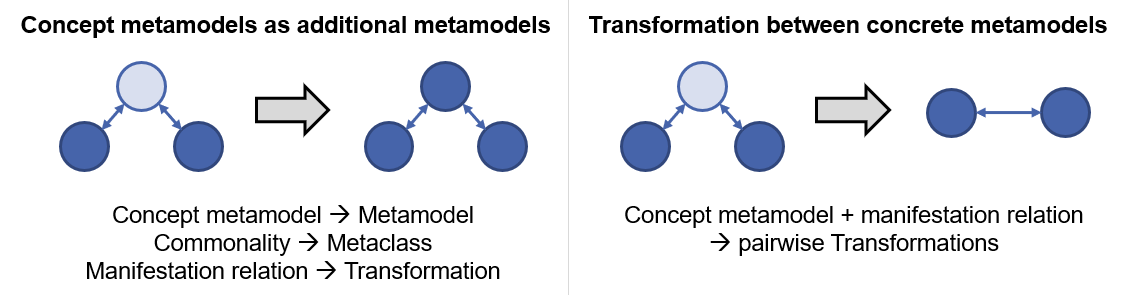
\includegraphics[width=\textwidth]{figures/quality/improvement/operationalization_alternatives.png}
    \caption[Alternatives for \commonalities operationalization]{Exemplification of alternatives to operationalize \commonalities specifications by using \conceptmetamodels (such as $\metamodel{C}{}$) as ordinary metamodels or by deriving direct transformations between the \concretemetamodels (such as $\metamodel{A}{}$ and $\metamodel{B}{}$) from them.}
    \label{fig:improvement:operationalization_alternatives}
\end{figure}

\mnote{Deriving executable transformations}
Up to now, we have discussed how to express consistency by means of \conceptmetamodels with \commonalities and manifestation relations in the \commonalities approach.
To actually preserve consistency of instances of the \concretemetamodels, such a specification must also be operationalized, such that executable transformations that can be applied after changes to these models are present or derived.
%\mnote{Operationalization options}
We can distinguish the following two basic options for this operationalization, which are also depicted in \autoref{fig:improvement:operationalization_alternatives}.
\begin{properdescription}
    \item[\ConceptMetamodels as Additional Metamodels:] The \conceptmetamodels are considered as ordinary metamodels and manifestation relations as ordinary transformations. Thus, we consider a transformation network of concrete and \conceptmetamodels, whose instances are kept consistent by transformations for the manifestation relations.
    \item[Transformations between \ConcreteMetamodels:] \Conceptmetamodels and manifestation relations are only used as auxiliary specification artifacts from which direct transformations between the \concretemetamodels are derived. For example, from the object-oriented design \conceptmetamodel in \autoref{fig:improvement:one_commonality_example}, a transformation between Java and the \gls{UML} is derived.
\end{properdescription}

\mnote{\Conceptmetamodels as ordinary metamodels}
The benefit of treating \conceptmetamodels as ordinary, additional metamodels and the manifestation relations as transformations is easy achievability.
No specific languages or generators are required to derive the necessary artifacts, but existing tools for defining metamodels and transformations can be used to define \conceptmetamodels and manifestation relations that can be readily used to preserve consistency of their instances.
A drawback of this approach is that it requires the management and persistence of additional artifacts, namely the instances of the \conceptmetamodels, which are only auxiliary artifacts that should not be visible to the user.
Hiding these artifacts can be achieved with an according framework, such that developers are still only confronted with the models of the tools they use.
Such functionality is provided by tools like \vitruv~\owncite{klare2021Vitruv-JSS} (see \autoref{chap:foundations:multiview:vitruv}) providing only views on instances of \concretemetamodels.

\mnote{Deriving direct transformations}
Deriving transformations between \concretemetamodels from a specification of \conceptmetamodels and manifestation relations benefits from not introducing further artifacts, such that a developer still only has to deal with instances of the \concretemetamodels he or she is concerned with.
This approach, however, suffers from reduced expressiveness, because not all multiary relations as expressed across additional \conceptmetamodels (see~\cite{diskin2018MultiModelSynchronization-FASE}) can be expressed by sets of binary relations and transformations preserving them~\cite{stevens2020BidirectionalTransformationLarge-SoSym}.
In addition, it requires the implementation of generators that derive transformations from specifications of \conceptmetamodels and manifestation relations.

\mnote{Correctness of derived transformation network}
Although with the second approach of deriving ordinary transformations the resulting transformation network contains cycles and does thus not provide correctness guarantees due to its topology, it still provides the guarantee due to the transformations being generated from a specification that ensures correctness.
For example, since a specification of \commonalities cannot contain incompatibilities, the derived transformations cannot contain them either, as long as the generator produces transformations that actually preserve consistency conforming to the defined manifestation relations.

\mnote{Multiple transformation executions}
For the orchestration of the generated transformations, no matter whether they are defined between \conceptmetamodels or derived between the \concretemetamodels, it is still necessary to allow the execution of each transformation multiple times.
Due to the situations identified in \autoref{chap:orchestration}, in which it is necessary to execute transformations multiple times to \enquote{negotiate} a result and repeatedly react to the changes of other transformations, such a behavior is still relevant for the \commonalities approach.
For example, propagating a class from Java across the object-oriented design \conceptmetamodel and the component-based design \conceptmetamodel to a component in the \gls{PCM} can lead to further additions to the class as soon as it is identified as a representation of a component, which then needs to be propagated back to the class representation in Java.
To support this, transformations should still be synchronizing and thus allowed to modify both involved models to support such situations that require this backpropagation of changes.

